\documentclass{article}
\usepackage{pdflscape}
\usepackage[margin=1in]{geometry}
\usepackage{verbatim}
\usepackage{graphicx, float}
\usepackage{makecell}
\usepackage{amsmath}
\usepackage{amsfonts}
\usepackage{amssymb}
\usepackage{hyperref}

\author{Astrid Augusta Yu}
\title{CPE 233 Lab \#4 -- MCU Generation Units}
\date{\today}

\DeclareMathOperator\bit{bit}
\DeclareMathOperator\byte{byte}
\DeclareMathOperator\word{word}

\begin{document}
\maketitle
\tableofcontents

\section{Questions}

\begin{enumerate}
    \item \textbf{There are five non-nop instructions in the sample program. Each of these instructions includes a comment that contain an “equation of importance”, which you used in this experiment to prove that your hardware was working correctly. For this question completely and explicitly explain how that desired value on the right side of the equation was formed relative to the given program. }

        \begin{tabular}{r l l}
            12 & \texttt{jal    x0,dog       } & \texttt{\# jal addr     =   8   (J-type test)          }\\
            && dog is at instruction \#2, or address \#8. \\ \\
            16 & \texttt{jalr   x0,-8,x20    } & \texttt{\# jalr addr    =   4   (I-type test) x20=rs1  }\\
            && This command points to address rs1$- 8 = 12 - 8 = 4$.  \\ \\
            20 & \texttt{beq    x10,x10,cat  } & \texttt{\# branch addr  =   4   (B-type test)          }\\
            && cat is at address 4.\\ \\
            24 & \texttt{sw     x10,12(x20)  } & \texttt{\# S-type immed =  12   (S-type test) x20=rs1  }\\
            && This is simply the immediate value (12) of the instruction. \\ \\
            28 & \texttt{lui    x0,255       } & \texttt{\# U-type immed =  0x000FF000 (U-type test)    }\\
            && $255=0xFF$ and lui loads it into the upper 20 bits by essentially \\
            &&padding the lower 20 bits with 12 0's. 
        \end{tabular}
    \item \textbf{The stack is a useful “mechanism” in MCUs and is referred to as an “abstract data type”. Define ADT in your own words and in the context of computer hardware.}
    
        An abstract data type is a generic mechanism used for storing data. It is defined to have a certain set of operations that operate 
        predictably, independent of the actual implementation. 
    \item \textbf{There is obviously no “stack” module in the RISC-V MCU architecture diagram. Where exactly is the stack then on the RISC-V MCU?  }
    
        The stack is inside the memory, at the very end. It grows to lower addresses and shrinks to higher addresses. The stack pointer is
        used to access the data, and pushing and popping is 
        done by subtracting and adding its position respectively.
    \item \textbf{The stack is well-known for push and pop operations, but there are no push and pop instructions in the RISC-V ISA. Show the two versions of how push and pop operations are implemented using the RISC-V ISA (show two set of code for each the push and pop operations).  }

        \begin{tabular}{r | c c}
            & Push & Pop \\
            \hline
            \hline
            Set 1 & \begin{tabular}{l}
                addi sp, sp, -4\\
                sw [reg], 0(sp)
            \end{tabular} & 
            \begin{tabular}{l}
                lw [reg], 0(sp) \\
                addi sp, sp, 4
            \end{tabular} \\
            \hline
            Set 2 & \begin{tabular}{l}
                sw [reg], -4(sp) \\
                addi sp, sp, -4
            \end{tabular} & 
            \begin{tabular}{l}
                addi sp, sp, 4 \\
                lw [reg], -4(sp) 
            \end{tabular} 
        \end{tabular}
    \item \textbf{The stack grows in the direction of lower addresses by convention. Change you code (for both push and pop) in the previous question to have the stack grow in the direction of higher addresses.  }

        \begin{tabular}{r | c c}
            & Push & Pop \\
            \hline
            \hline
            Set 1 & \begin{tabular}{l}
                addi sp, sp, 4\\
                sw [reg], -4(sp)
            \end{tabular} & 
            \begin{tabular}{l}
                lw [reg], -4(sp) \\
                addi sp, sp, -4
            \end{tabular} \\
            \hline
            Set 2 & \begin{tabular}{l}
                sw [reg], 0(sp) \\
                addi sp, sp, 4
            \end{tabular} & 
            \begin{tabular}{l}
                addi sp, sp, -4 \\
                lw [reg], 0(sp) 
            \end{tabular} 
        \end{tabular}
    \item \textbf{The stack is used for “general data storage”, but it’s specifically used to store information in two scenarios. What are those scenarios and what information does it store?  }

    It typically stores information upon calling a subroutine.
    \item \textbf{The RISC-V OTTER has 32 “general purpose” registers. Why is it that that RISC-V OTTER programmers should never use registers x1 and x2?  }

    x1 is the return address, and x2 is the stack pointer.
    \item \textbf{What does the stack pointer point at?  }
    
    It points at the item at the top of the stack.
    \item \textbf{Stack overflow and underflow are a major issue in assembly language programs. Briefly explain why these conditions major issues? }

    \includegraphics[width=\linewidth]{stack.png}

    \item \textbf{We keep saying that subroutines need to closely match their call/return instruction and push/pop instruction pairs. Briefly explain why this is important.  }

    The registers must be pushed one way and popped the other way because the stack is a LIFO data structure.  
    If t0 and t1 are pushed in that order, then also popped in that order, what will happen is that their values will be swapped. 
    However, if t0 then t1 are pushed and t1 then t0 are popped, then they will have the values.
\end{enumerate}

\pagebreak

\section{Programming Assignment}

\textbf{Write a RISC-V OTTER assembly language subroutine that converts a binary value in register x10 to a 4-digit BCD stored in the lower four nibbles of register x11. The binary value will never be greater than 9999. Make sure your subroutine does not permanently change any registers other than x11. }

\begin{verbatim}
.text

# This section exists to test the subroutine.
main:
    li x10, 1234
    call bcd

    li x10, 10
    call bcd

    li x10, 0
    call bcd

    li x10, 3483
    call bcd

    li x10, 13
    call bcd

    li x10, 69
    call bcd

    li x10, 832
    call bcd
    j end

#----------------------------------------------------------------
#- Converts a value less than 10000 into its 4-digit BCD 
#- representation.
#-
#- Parameters
#-      a0/x10 - value to convert
#- Returns
#-      a1/x11 - BCD representation
#- Tweaked registers - x11
#---------------------------------------------------------------- 
bcd:
    # t0 is the register used for accumulating the BCD.
    addi sp, sp, -16
    sw t0, 0(sp)
    sw a0, 4(sp)
    sw a2, 8(sp)
    sw ra, 12(sp)

    mv a1, a0       # Dividend
    li a2, 1000     # Divisor
    call divide     # a0 R a1 = a1 / a2

    mv t0, a0       # Quotient = thousands digit.
    slli t0, t0, 4  # Shift BCD

    li a2, 100      # Divisor. Modulus = new dividend.
    call divide     # a0 R a1 = a1 / a2

    or t0, t0, a0   # Quotient = hundreds digit.
    slli t0, t0, 4  # Shift BCD.
    
    li a2, 10       # Divisor. Modulus = new dividend.
    call divide     # a0 R a1 = a1 / a2

    or t0, t0, a0   # Quotient = ten's digit.
    slli t0, t0, 4  # Shift BCD.
    or t0, t0, a1   # Modulus = one's digit.

    mv a1, t0       # Return value

    lw t0, 0(sp)
    lw a0, 4(sp)
    lw a2, 8(sp)
    lw ra, 12(sp)
    addi sp, sp, 16

    ret

#----------------------------------------------------------------
#- Implementation of binary division. Given a dividend n and 
#- divisor p, runs in approximately log(n / p) time.
#-
#- Parameters
#-      a1 - dividend
#-      a2 - divisor
#- Returns
#-      a0 - quotient
#-      a1 - modulus/remainder
#- Tweaked registers - a0, a1
#----------------------------------------------------------------
divide:
    blt a1, a2, iszero  # If dividend < divisor return early

    # Store registers on stack
    addi sp, sp, -8
    sw t0, 0(sp)
    sw a2, 4(sp)

    # Initialize registers
    li t0, 1  # divisor coefficient

expand:  # Double the divisor until it is greater than dividend
    slli t0, t0, 1
    slli a2, a2, 1
    bgt a1, a2, expand

    li a0, 0  # quotient
subtractloop:  # Halve the divisor until we go under the original value
    srai t0, t0, 1
    bne zero, t0, subtractloop
    srai a2, a2, 1
    blt a1, a2, nosub
subtract:
    # Add to quotient if divisor falls below modulus/dividend
    or a0, a0, t0
    sub a1, a1, a2
nosub:
    j subtractloop

    lw t0, 0(sp)
    lw a2, 4(sp)
    addi sp, sp, 8
    ret
iszero:
    li a0, 0
    ret

end:
\end{verbatim}

\section{Hardware Design Assignment}
\textbf{Show a block diagram that you could use to solve the following problems. Circuits such as MCUs generally have “register files”, which are nothing more than “dual port RAMs”. This implies that you can read from two different addresses at the same time, and write to one address. This should seem familiar as it is the way the RISC-V instructions work. For this problem, design a dual-port RAM using two single port RAMs (such as the RAMs you’ve been working with up to this point). Writing to the RAMs should be synchronous and reading from the RAMs should be asynchronous. Include the top two levels of BBDs for your design. Make the dual port RAM should be 32x32, which is the same capacity as the register file that the RISC-V uses. }

See next page for my solution.

\begin{landscape}
\centering
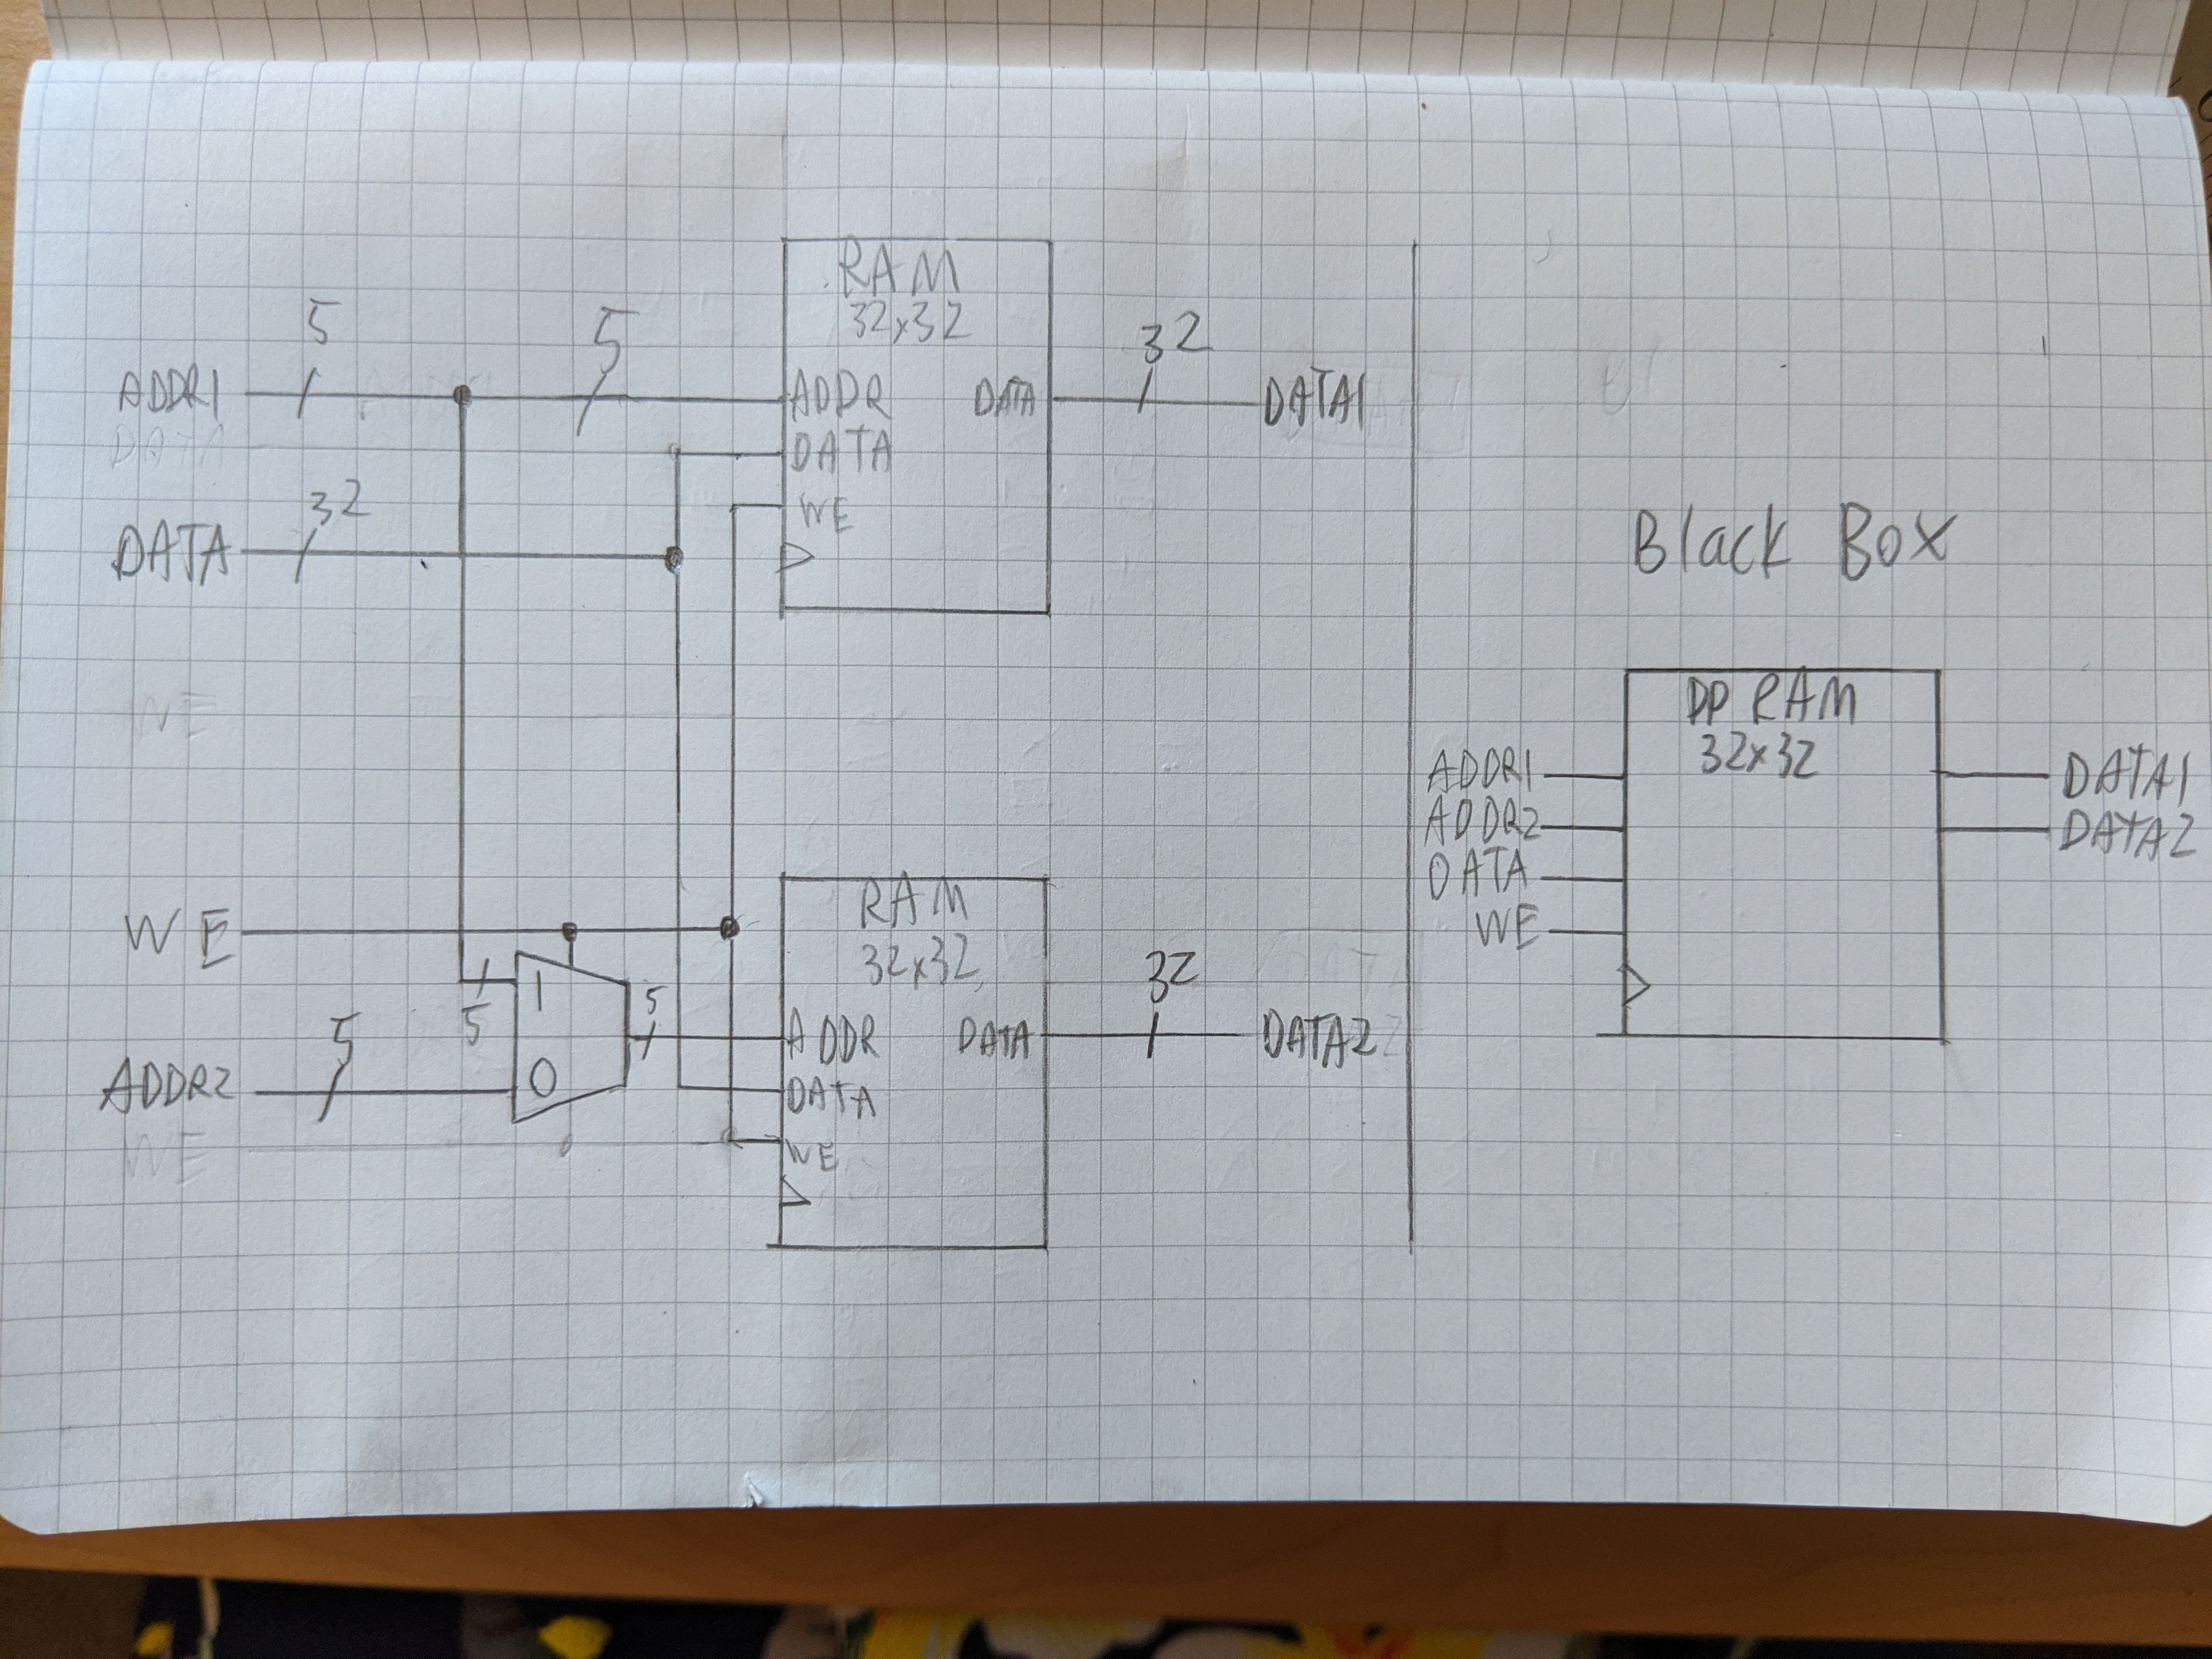
\includegraphics[width=0.95\linewidth]{hw.jpg}
    
\end{landscape}

\section{HDL Code}

\subsection{Immediate Value Generator}

\begin{verbatim}
`timescale 1ns / 1ps
//////////////////////////////////////////////////////////////////////////////////
// Company: Cal Poly
// Engineer: Astrid Yu
// 
// Create Date: 04/24/2020 04:20:00 PM
// Design Name: Immediate Value Generator
// Module Name: immed_gen
// Project Name: Otter MCU
// Target Devices: 
// Tool Versions: 
// Description: 
// 
// Dependencies: 
// 
// Revision:
// Revision 0.01 - File Created
// Additional Comments:
// 
//////////////////////////////////////////////////////////////////////////////////


module ImmedGen(
    input [31:7] ir,
    output [31:0] b_type_imm,
    output [31:0] j_type_imm,
    output [31:0] i_type_imm,
    output [31:0] s_type_imm,
    output [31:0] u_type_imm
    );
    
    logic isbj_sign;
    assign isbj_sign = ir[31];
    
    assign i_type_imm = {{21{isbj_sign}}, ir[30:25], ir[24:20]};
    assign s_type_imm = {{21{isbj_sign}}, ir[30:25], ir[11:7]};
    assign b_type_imm = {{20{isbj_sign}}, ir[7], ir[30:25], ir[11:8], 1'b0};
    assign u_type_imm = {ir[31:12], 12'b0};
    assign j_type_imm = {{12{isbj_sign}}, ir[19:12], ir[20], ir[30:21], 1'b0};
endmodule    
\end{verbatim}

\pagebreak

\subsection{Branch Address Generator}
\begin{verbatim}
`timescale 1ns / 1ps
//////////////////////////////////////////////////////////////////////////////////
// Company: Cal Poly
// Engineer: Astrid Yu
// 
// Create Date: 04/24/2020 04:20:00 PM
// Design Name: Branch Address Generator
// Module Name: branch_addr_gen
// Project Name: Otter MCU
// Target Devices: 
// Tool Versions: 
// Description: 
// 
// Dependencies: 
// 
// Revision:
// Revision 0.01 - File Created
// Additional Comments:
// 
//////////////////////////////////////////////////////////////////////////////////


module BranchAddrGen(
    input [31:0] pc,
    input [31:0] rs,
    input [31:0] b_type_imm,
    input [31:0] i_type_imm,
    input [31:0] j_type_imm,
    output [31:0] jal,
    output [31:0] branch,
    output [31:0] jalr
    );
    
    assign jal = pc + j_type_imm;
    assign branch = pc + b_type_imm;
    assign jalr = rs + i_type_imm;
    
endmodule    
\end{verbatim}

\begin{landscape}
\section{Simulation Results}
\subsection{Waveform Output}
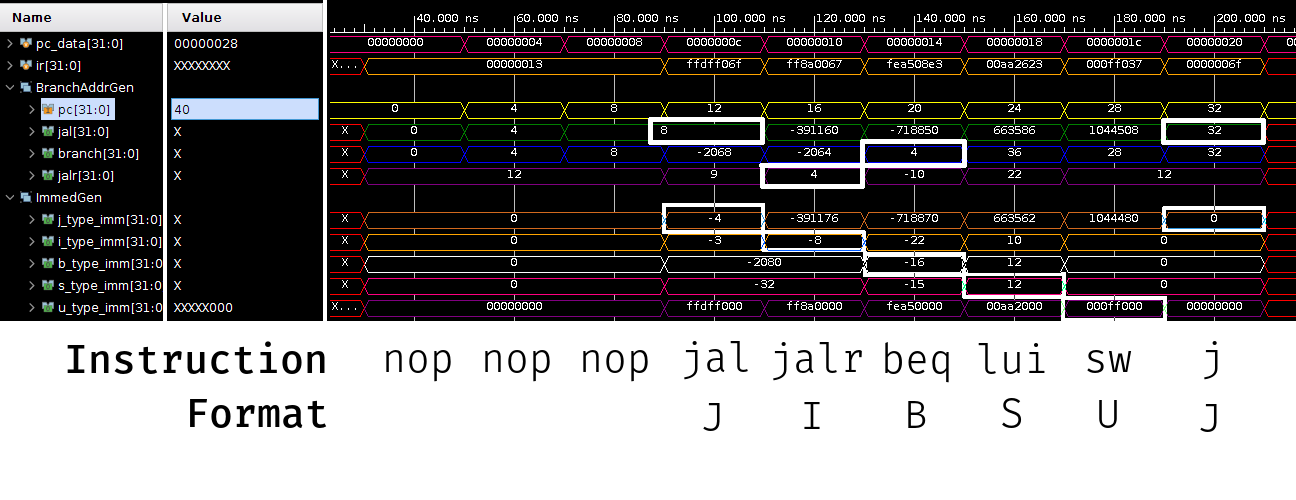
\includegraphics[width=\linewidth]{wer.png}

\subsection{Table of Outputs}
\centering
\begin{tabular}{r | r l || c | c || c | c }
    &&& \textbf{Format} & \textbf{Immediate} & \textbf{AddrGen Type} & \textbf{Address} \\
    \hline
    0  & & \texttt{nop} & --- & --- & --- & --- \\
    4  & cat: & \texttt{nop} & --- & --- & --- & --- \\
    8  & dog: & \texttt{nop} & ---& --- & --- & --- \\
    12 & & \texttt{jal    x0,dog       } & J & -4 & jal & 8 \\
    16 & & \texttt{jalr   x0,-8,x20    } & I & -8 & jalr & 4 \\
    20 & & \texttt{beq    x10,x10,cat  } & B & -16 & branch & 4 \\
    24 & & \texttt{sw     x10,12(x20)  } & S & 12 & --- & --- \\
    28 & & \texttt{lui    x0,255       } & U & 0x000FF000 & --- & ---\\
    32 & end:& \texttt{j      end}       & J & 0 & jal & 0 \\
\end{tabular}
\end{landscape}
    
\end{document}